\documentclass{standalone}
\usepackage{tikz}
\usetikzlibrary{decorations.pathreplacing}
\usepackage{amsfonts}

\begin{document}
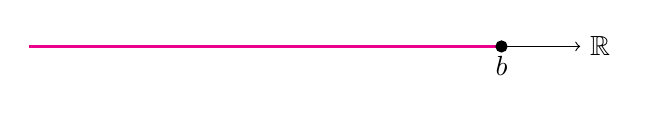
\begin{tikzpicture}
% Draw the real line
  \draw[->] (-3.5,0) -- (3.5,0) node[right] {$\mathbb{R}$};
  
  
  
    % Draw the magenta segment between '-y' and 'y' and make it thicker
  \draw[magenta, line width=1pt] (-3.5,0) -- (2.44,0);
  
  
  % Draw the point 'x' and '0'


  \filldraw (2.5,0) circle (2pt) node[below] {$b$};



  
  \end{tikzpicture}
\end{document}